\section{ACOS Inverse Trigonometric Arccosine Function}

\subsection{Usage}

Computes the \verb|acos| function for its argument.  The general
syntax for its use is
\begin{verbatim}
  y = acos(x)
\end{verbatim}
where \verb|x| is an \verb|n|-dimensional array of numerical type.
Integer types are promoted to the \verb|double| type prior to
calculation of the \verb|acos| function.  Output \verb|y| is of the
same size and type as the input \verb|x|, (unless \verb|x| is an
integer, in which case \verb|y| is a \verb|double| type).  
\subsection{Function Internals}

Mathematically, the \verb|acos| function is defined for all 
arguments \verb|x| as
\[
 \mathrm{acos} x \equiv \frac{pi}{2} + i \log \left(i x + 
  \sqrt{1-x^2}\right).
\]
For real valued variables \verb|x| in the range \verb|[-1,1]|, the function is
computed directly using the standard C library's numerical \verb|acos|
function. For both real and complex arguments \verb|x|, note that generally
\[
  \mathrm{acos}(\cos(x)) \neq x,
\]
\subsection{Example}

The following code demonstates the \verb|acos| function over the range 
\verb|[-1,1]|.
\begin{verbatim}
--> t = linspace(-1,1);
--> plot(t,acos(t))
\end{verbatim}


\centerline{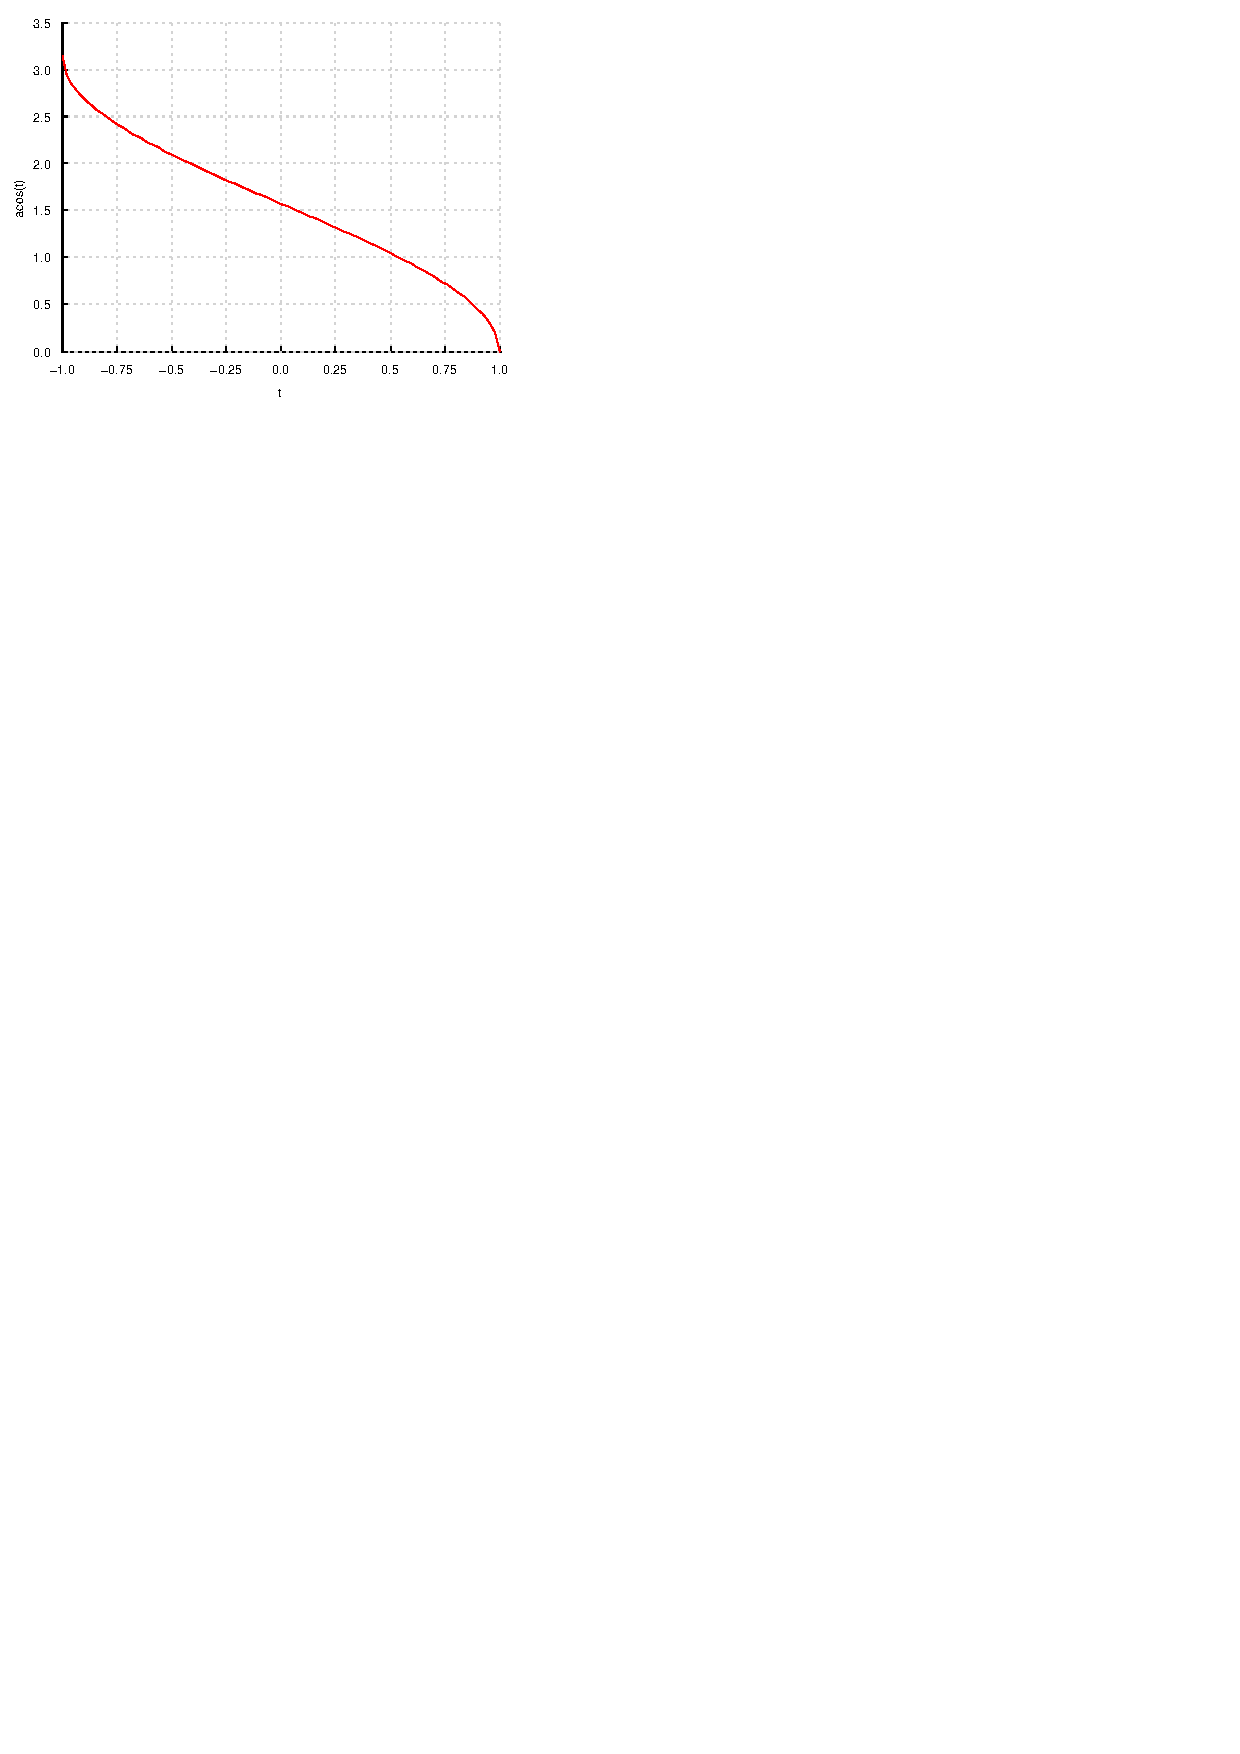
\includegraphics[width=8cm]{acosplot}}

